\section{Research Objective 2: Develop data-parallel methods for evaluating Boolean circuits}
\begin{frame}
    \Large{\centerline{\textbf{Research Objective 2}}}
    \vspace{6pt}
    \large{\centerline{\textbf{Develop data-parallel methods for evaluating Boolean circuits}}}
\end{frame}

%% ------------------------------------------------------------------
%% From Truth Table to Bit-Parallelism
%% ------------------------------------------------------------------
\subsection{Bitwise Kernels}
\begin{frame}{Boolean Truth Table – Single Bit}
\centering
\begin{tabular}{c|c|c|c|c|c|c|c}
$X$ & $Y$ & AND & OR & XOR & NAND & NOR & XNOR \\ \hline
0 & 0 & 0 & 0 & 0 & 1 & 1 & 1 \\
0 & 1 & 0 & 1 & 1 & 1 & 0 & 0 \\
1 & 0 & 0 & 1 & 1 & 1 & 0 & 0 \\
1 & 1 & 1 & 1 & 0 & 0 & 0 & 1 \\
\end{tabular}
\vspace{8pt}
\begin{itemize}
  \item Classical gate evaluation operates \emph{bit-by-bit}.  Throughput $\propto$ number of Boolean operations.
  \item Perform \textbf{64} of these truth-table lookups in one machine instruction.
\end{itemize}
\end{frame}

%% ------------------------------------------------------------------
%% Eight Bits in Parallel
%% ------------------------------------------------------------------
\begin{frame}{Extending to a 64-Bit Word}
\begin{columns}
  \column{0.55\textwidth}
    \begin{itemize}
      \item Pack 64 independent Bernoulli trials into one byte.
      \item Bitwise primitives act \emph{independently} on every bit position.
      \item Hardware native instructions guarantee ns latency.
    \end{itemize}
  \column{0.45\textwidth}
    \centering
    \includegraphics[height=0.7\textheight]{2_framework/research_objective_2_sycl_eval/bitwise_xy_inv.png}
\end{columns}
\end{frame}


% special case for k/n kernels
\begin{frame}[t]{Handling Voter Logic - Expansion} 
  \begin{columns}
    \column{0.60\textwidth}
    {
      \textbf{The Simplest Type of Query: Eval(G)}\par
      \begin{itemize}
          \item {Set the inputs [on/off].}
          \item {Observe the outputs [on/off].}
      \end{itemize}\par
      \vspace{2pt}
      \tiny{\textbf{\emph{{Can be used as a building block for an embedding ML model.}}}}\par
            \vspace{10pt}
      \normalsize\textbf{But how to handle K/N gates?}

    }
     \column{0.4\textwidth}
      \input{1_concepts/ft_3_of_5}\par % Replace with your image file
  \end{columns}
\end{frame}


%% ------------------------------------------------------------------
%% SYCL Execution Model
%% ------------------------------------------------------------------
\subsection{The SYCL Execution Model}
\begin{frame}{SYCL Execution Model in a Nutshell}
      \centering
      \includegraphics[width=0.9\textwidth]{2_framework/research_objective_2_sycl_eval/sycl.png}\par % Replace with your image file
\end{frame}

%% ------------------------------------------------------------------
%% SYCL Execution Model
%% -----------------------------------------------------------------

\begin{frame}{SYCL Execution Model in a Nutshell}
  \begin{columns}
    \column{0.3\textwidth}
      \tiny
      \begin{description}
        \item[Host] submits \texttt{queue.submit()} with a \texttt{kernel\_name}.
        \item[ND-Range] $\langle\,\text{global}\;3\!\times\!\text{local}\,\rangle$ defines grid.
        \item[Work-Group] maps to CUDA block / OpenCL work-group.
        \item[Sub-Group] (warp/wavefront) gives warp-level shuffle & ballot ops.
        \item[Device USM] used for persistent bit-packed buffers.
      \end{description}
    \column{0.7\textwidth}
      \centering
      \includegraphics[width=1\textwidth]{2_framework/research_objective_2_sycl_eval/sycl.png}\par % Replace with your image file
  \end{columns}
\end{frame}

%% ------------------------------------------------------------------
%% Mapping PDAG Layers to Kernels
%% ------------------------------------------------------------------
\subsection{Kernel Execution}
\begin{frame}{Mapping PDAG Layers to SYCL Kernels}
    \tiny
  \begin{enumerate}
    \item Topological sort $\Rightarrow$ depth index $d$.
    \item All nodes with depth $d$ share \emph{identical fan-in length}.  \texttt{range<3>} := $(\text{batch},\text{gate},\text{bitpack})$.
    \item One kernel per layer; gate type dispatched via template specialization.
    \item Streams results to next-depth buffer in global memory.
  \end{enumerate}
  \vspace{-42pt}
  \begin{columns}
      \column{0.6\textwidth}
        \centering
      \includegraphics[width=1\textwidth]{2_framework/research_objective_2_sycl_eval/sycl.png}
      \column{0.4\textwidth}
        \centering
        \includesvg[height=0.9\textheight]{1_concepts/dag_pass_2.svg}
  \end{columns}

\end{frame}

\begin{frame}{Eval Query Performance on Generic Backends}
\centering
        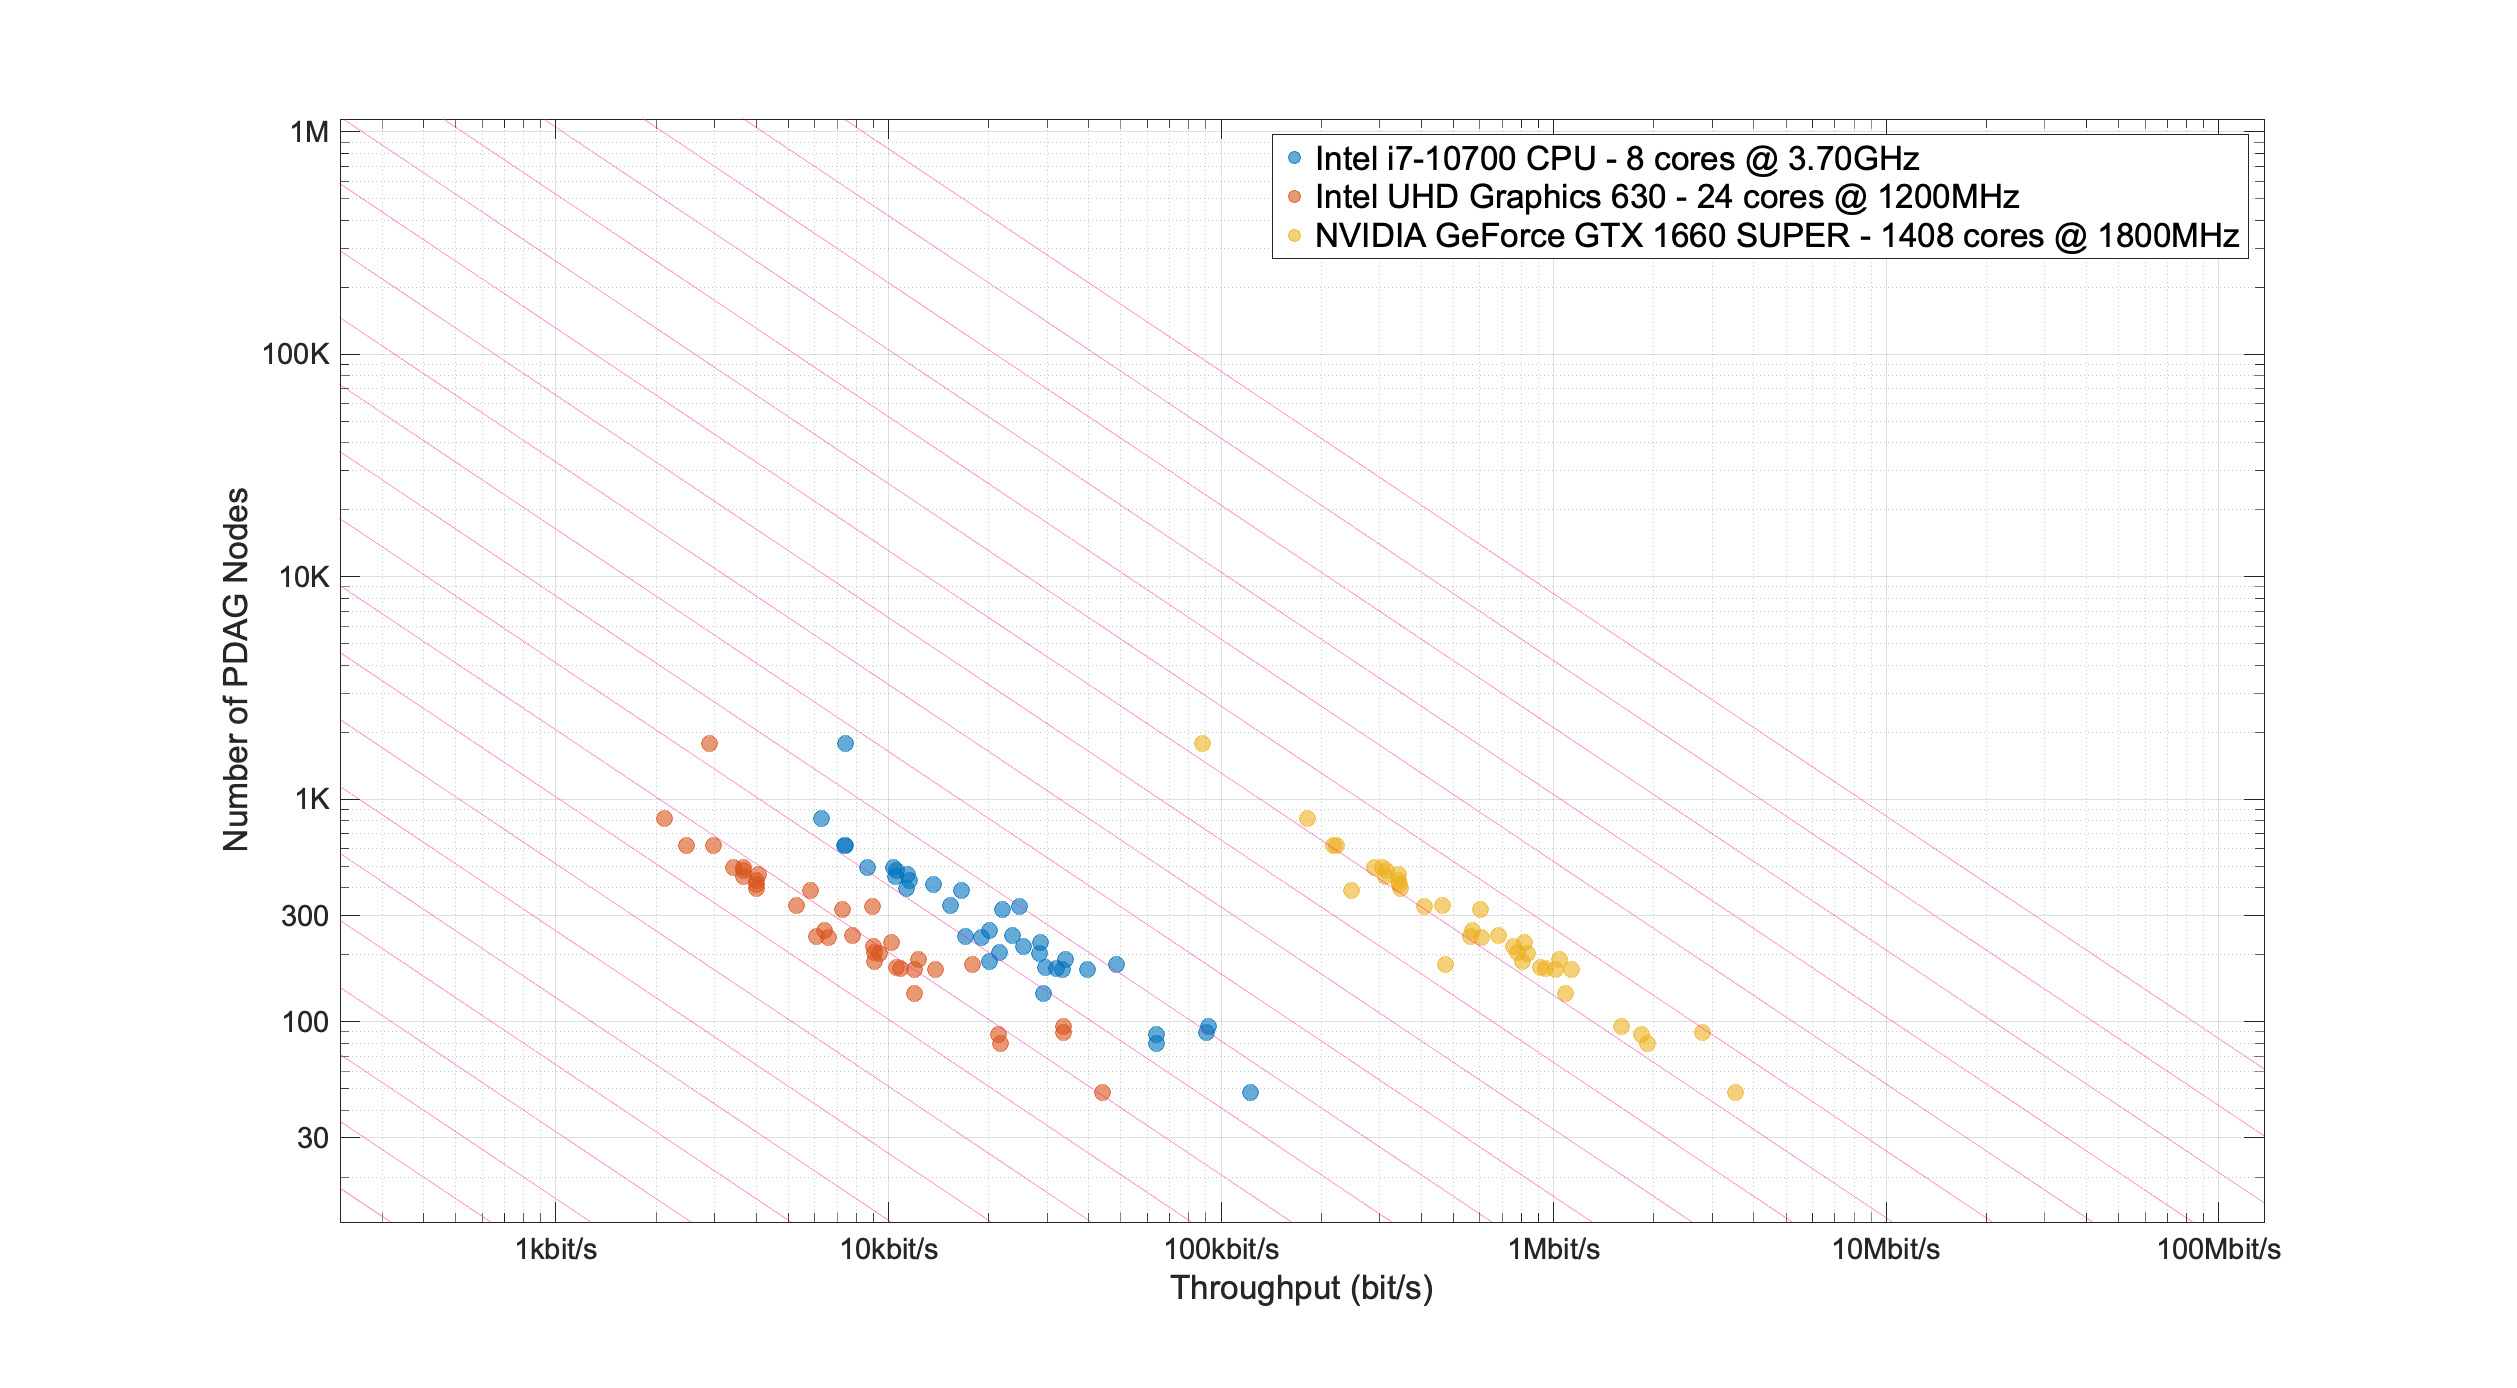
\includegraphics[height=0.9\textheight]{2_framework/research_objective_2_sycl_eval/slides_nodes_vs_throughput.eps}
\end{frame}

\begin{figure}[hb]
    \centering
    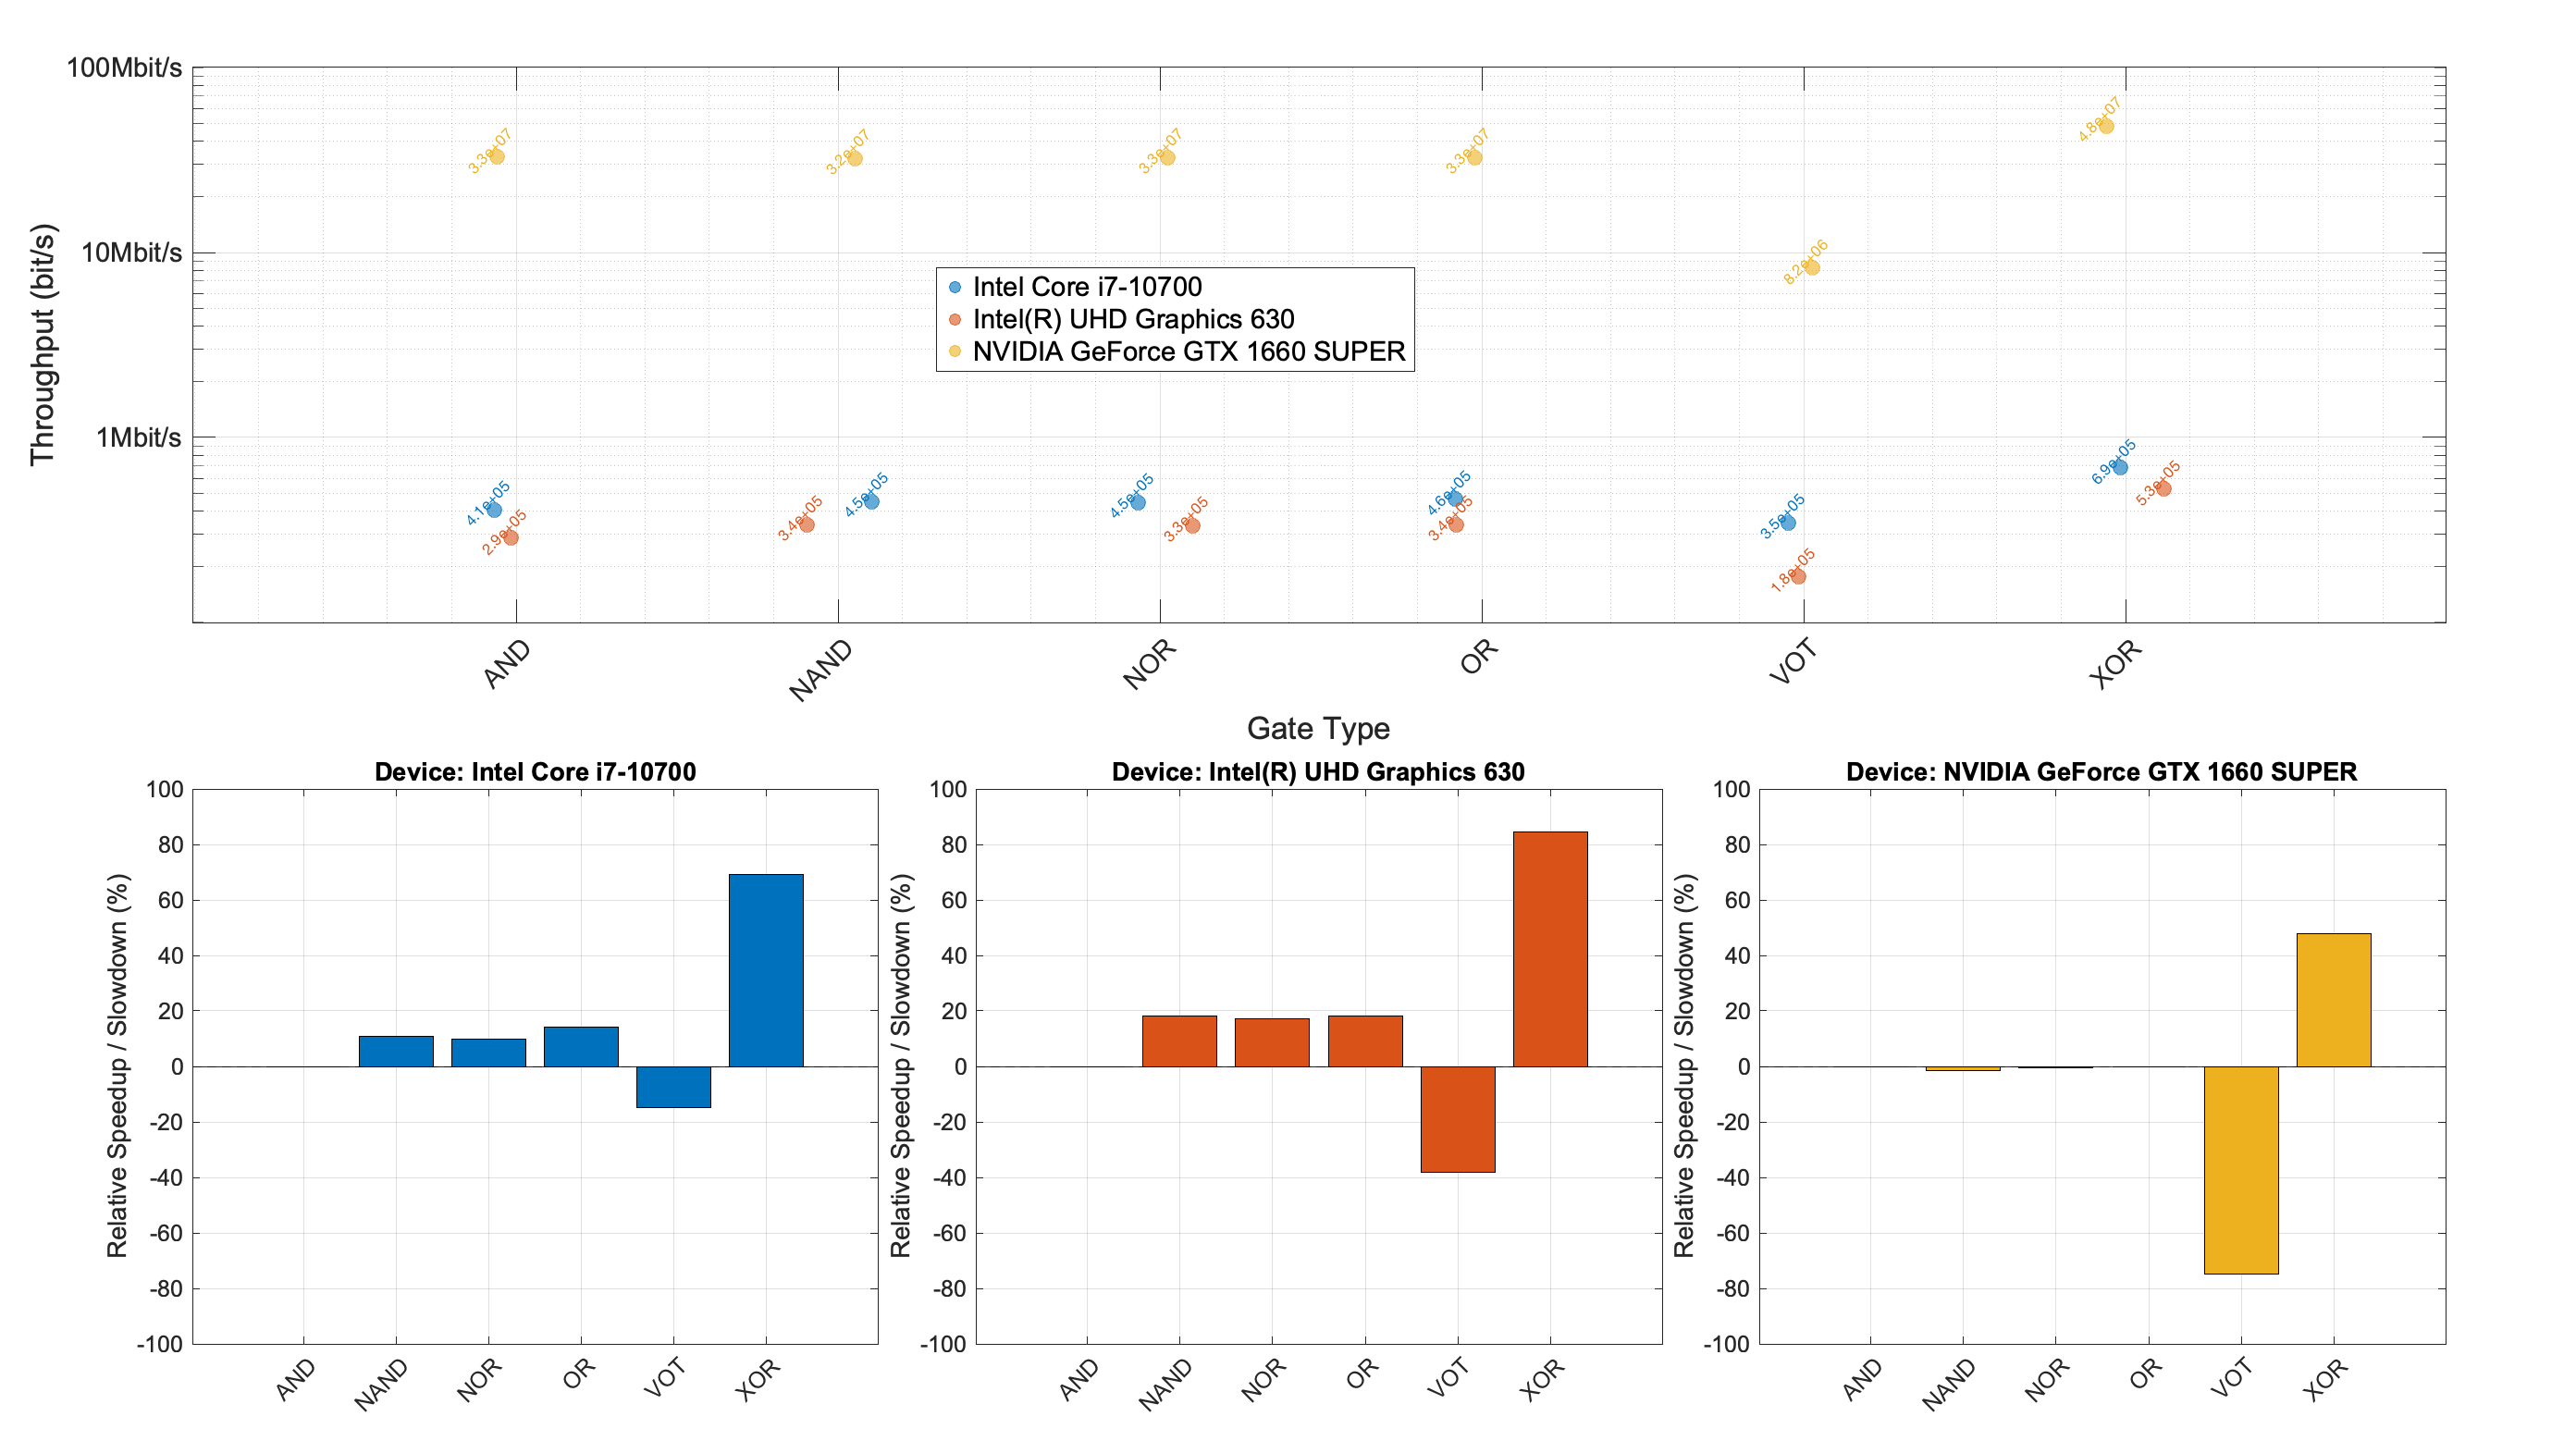
\includegraphics[height=0.8\textheight]{execution_model/slides_throughput_by_gate_type.eps}
    \caption{(Top) Throughput in bit/second on various backends for different gate types. (Bottom) \% Relative speedup/slowdown as compared to the AND gate.}
    \label{fig:gate_throughput}
\end{figure}

%% throughput graph
\begin{frame}{Eval Query Performance on Discrete GPUs}
  \begin{columns}
    \column{0.60\textwidth}
    {
      \begin{itemize}
          \item {Latency: 20-30 $ms$ per layer.}
          \item {Throughput: Graph depth and VRAM bound (see plot).}
          \item {Benchmarked on Nvidia GTX 1660 [6GB].}
          \item {Graph sizes: from $\approx 50$ to $\approx 2000$ nodes.}
          \item {Evals: from 16M to 1B per node per pass.}
      \end{itemize}
      \vspace{10pt}
      \textbf{Q: Are these enough samples to estimate the Expectation Query?}
    }
     \column{0.4\textwidth}
        \centering
        \includesvg[height=0.9\textheight]{1_concepts/mem_allocation_lines_zoom.svg}
  \end{columns}
\end{frame}



